\section{Diagnostic Methods Supplemental Information}

\subsection{Microwave Scattering}

The microwave scattering setup is shown in \ref{fig:SI_MWS_Setup_Silicon}. The parts were ordered from Erevant, formerly Sage Millimeter. The system is W-band and based on WR-10 waveguides. The microwave source is a 90 GHz Gunn oscillator (SOM-90305213-10-S1) with an output power of +13 dBm. The output of this source is fed into a 10 dB gain, +15 dBm P1dB, in-line waveguide power amplifier (SBP-7531141015-1010-E1). The output of the power amplifier is then fed into a 4-way in-line power divider (SWP-90310404-10-E1). In the current configuration, only two outputs of the power divider are used, and the remaining two are terminated with waveguide terminators (TODO). One power of the power divider is used for the main transmitted power, which is sent through waveguides to a horn (TODO) that transmits the microwaves into free space. The transmitted microwaves after the sample are collected by the same type of horn, and the collected microwaves are sent to the IQ mixer (SFQ-75311415-1010SF-N1-M). The LO input of the IQ mixer is fed by the remaining port of the power divider. Between the power divider and the LO input there is a phase shifter (STP-18-10-M2) that is typically used to maximize the I signal in the absence of a sample. 

The I and Q signals from the oscilloscope are fed directly into a Teledyne Leroy oscilloscope (TODO). The oscilloscope utilized 1 MOhm impedance. (TODO) The oscilloscope is triggered from the excimer laser. 

\begin{figure}[]
\centering
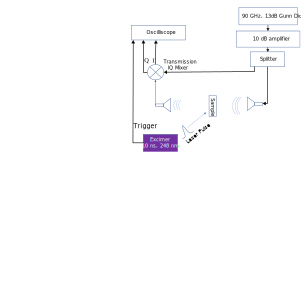
\includegraphics[width=0.8\textwidth]{\repodir/final/figures/SI/output/MWS_Setup_Silicon.png}
\caption{Microwave scattering setup for silicon wafers.}
\label{fig:SI_MWS_Setup_Silicon}
\end{figure}

\begin{figure}[]
\centering
\includegraphics[width=0.8\textwidth]{\repodir/final/dataset/output/figures/mws_nothing_T0.png}
\caption{A) Measurement of transmission without any torch, B) position dependent transmission measurement.}
\label{fig:SI_MWS}
\end{figure}


\begin{figure}[]
\centering
\includegraphics[width=0.8\textwidth]{\repodir/final/dataset/output/figures/mws_nothing_time_trace_2023-05-18.png}
\caption{Time trace from 2023-05-18 of the transmission measurement without any free jet.}
\label{fig:SI_MWS}
\end{figure}

\ref{fig:SI_mws_processing_overview} shows the processing steps for the MWS data. 



\begin{figure}[]
\centering
\includegraphics[width=0.8\textwidth]{\repodir/experiment/analysis/mws/output/figures/mws_processing_overview.png}
\caption{Microwave processing overview}
\label{fig:SI_mws_processing_overview}
\end{figure}

\begin{figure}
\centering
\includegraphics[width=0.8\textwidth]{\repodir/experiment/analysis/mws/resampling/output/figures/mws_sample_nors_compare.png}
\caption{Comparison of the resampling methods.}
\label{fig:SI_mws_resampling}
\end{figure}


\begin{figure}
\centering
\includegraphics[width=0.8\textwidth]{\repodir/experiment/analysis/mws/output/figures/mws_fitting_compare.png}
\caption{Comparison of the fitting methods for the monomolecular regime. Fit to an exponential model and full solution of differential equation. }
\label{fig:SI_mws_fitting_compare}
\end{figure}

\subsection{Laser Profile}


\begin{figure}[]
\centering
\includegraphics[width=0.8\textwidth]{\repodir/experiment/analysis/mws/output/figures/laser_profile.png}
\caption{Laser profile measurement}
\label{fig:SI_Laser_Profile}
\end{figure}

\subsection{AES}
\begin{figure}[]
    \centering
    \includegraphics[width=0.8\textwidth]{\repodir/experiment/analysis/absem/output/figures/absem_proc_overview.png}
    \caption{AES processing overview}
    \label{fig:SI_AES_proc_overview}
\end{figure}
